\chapter{Compiling and Linking}

Compiling the feed handler as a shared library and as a standalone executable requires different
steps and build artefacts. How you structure your code and build your software can differ based
on the platform that your are running on. The example code that is provided alongside this document
has been written to compile on both Windows and Linux platforms using the CMake build tool which
abstracts some of these details away. We will describe how to build these objects manually for
each platform to highlight some of the requirements specific to each. We will indicate any potential
cross platform issues as we present code, and examples of how to work around these problems can be
found in the example source code.

The first file you will need to download from the Kx subversion repository is the \verb|"k.h"| 
header\footnote{http://code.kx.com/svn/kx/kdb+/c/c/k.h}. You should include this header whenever you
need to interface with kdb+ as it defines all of the types and functions that are necessary. The same
header file is used with both version \textbf{2.x} and \textbf{3.x} of kdb+ and the version is selected
by defining \verb|KXVER| to be either \textbf{2} or \textbf{3}. If \verb|KXVER| is not defined, the
compiler should emit an error to notify you of this.

\begin{figure}[h]
\begin{lstlisting}[language=C]
#include <stdlib.h>
#include <stdio.h>

#define KXVER 3 // declaring that we want to work with v3.x of kdb+
#include "k.h"

int main(void)
{
	return EXIT_SUCCESS;
}
\end{lstlisting}
\caption{Importing the "k.h" header and defining KXVER in a C program}
\end{figure}

It is usually possible to define \verb|KXVER| from your build tools when compiling, but this differs
depending on the platform and tools. As an example, on Linux with GCC, we could use the \textbf{-D} flag
to specify \verb|KXVER| instead of using the preprocessor.

\begin{figure}[h]
\begin{lstlisting}
gcc example.c -DKXVER=3 -fpic -shared -std=gnu99 -o example.so
\end{lstlisting}
\caption{Defining KXVER from the command line with GCC}
\end{figure}

All of the example code in this document assumes that a more recent version of C is used in order to provide
some quality of life improvements in the code (e.g. declaring iteration variables inside the for loop). \textbf{Visual Studio} provides a C++ compiler that supports these features out of the box. Standard C
compilers such as \textbf{GCC} and \textbf{clang} will require a flag to enable these features 
(e.g. \textit{(-std=gnu99)}).

It should be noted that not all functions declared in \verb|"k.h"| are available to both libraries and
executables. An example of this is the \textbf{sd0} and \textbf{sd1} functions which are covered later
in the document (it wouldn't make sense for these functions to exist inside a standalone executable).

\section{Linux}

\subsection{Shared Objects}

On Linux, you can create a shared object by simply passing the \textbf{-shared} flag when compiling. This
will create a \textbf{.so} file that exports any functions that are not prefixed with the \textit{static}
keyword. It is also important that the binary produced is position independent if it is to be shared between
multiple processes, so you should also use the \textbf{-fpic} flag when compiling a shared library.

\begin{figure}[h]
	\begin{lstlisting}
	gcc example.c -fpic -shared -std=gnu99 -o example.so
	\end{lstlisting}
	\caption{Compiling a position independent shared library with GCC}
\end{figure}

You do not need to link against any other objects in order to build or load the library on Linux. To check
that the correct functions have been exported, you can use tools such as \textbf{objdump} to inspect the binary
and view the symbol tables. Passing objdump the \textbf{-t} flag will make it print the symbol tables to the console,
and you can look for your function name in the rightmost column of the output.

\begin{figure}[h]
	\begin{lstlisting}
	aquaq@localhost:~/fakefeed/bin> objdump -t example.so
	
	example.so:     file format elf64-x86-64
	
	SYMBOL TABLE:
	...
	0000000000000960 g     F .text	00000000000000d6              GenerateCore
	0000000000000b10 g     F .text	000000000000008d              GenerateTrade
	0000000000000a40 g     F .text	00000000000000c2              GenerateQuote
	...
	0000000000000ba0 g     F .text	0000000000000077              ProcessFeed
	0000000000000000       F *UND*	0000000000000000              time@@GLIBC_2.2.5
	00000000000007f8 g     F .init	0000000000000000              _init
	\end{lstlisting}
	\caption{Viewing the symbol table of a shared object using \textit{objdump}}
\end{figure}

One other issue you will need to take care of is that you want to make sure you are not building a 64 bit
shared library to load into a 32 bit q process or vice versa. This can be changed with the \textbf{-m32}
(for 32 bit) and \textbf{-m64} (for 64 bit) flags with GCC. Attempting to load a 64 bit shared object into
a 32 bit q process will cause an error to be thrown and the process may exit.

\subsection{Standalone Executable}

The process for creating a standalone executable that can interface with kdb+ is similar to building a shared
object. The key difference is that you will need to provide an entry point (i.e. define \verb|int main(...)|)
and also link against an object that defines the functions in \verb|"k.h"|. The reason that we didn't need to
link against an object for the shared library is that the q process itself will have already loaded them.

On Linux, the \textbf{c.o} file contains the implementations and is available in both \textbf{32-bit}\footnote{http://code.kx.com/svn/kx/kdb+/l32/} and \textbf{64-bit}\footnote{http://code.kx.com/svn/kx/kdb+/l64/} versions. It is critical that you load the correct
version of c.o to match the executable that you are building.

To build the executable, you just need to pass the \textbf{c.o} object alongside your code and make sure that
the \textbf{-shared} and \textbf{-fpic} flags are not defined. You will need
to link against the \textbf{pthread} library using \textbf{-lpthread} too as this is required for some of the
functions to execute correctly.

 \begin{figure}[h]
 \begin{lstlisting}
 gcc example.c c.o -std=gnu99 -lpthread -o example
 \end{lstlisting}
 \caption{Compiling an executable with GCC using the \textit{pthread} library}
 \end{figure}
 
 Similarly to the shared object, you can use the \textbf{-m32} and \textbf{-m64} flags with GCC in order to
 build 32-bit or 64-bit executables respectively. Linking against the wrong version of the c.o file can cause
 runtime errors or segfaults to occur. 
 
 \section{Windows}
 
 \subsection{Shared Objects}
 
 On Windows, it is typical to use a tool set such as \textbf{Visual Studio}, rather than the commandline tools (e.g \textbf{cl.exe}). We will show how to use both Visual Studio projects and the command line in order to compile the code.
 
 After creating your C++ project in Visual Studio, open the Property Pages and click on \verb|Configuration Properties -> General|. Make sure that the Configuration Type is set to \textbf{Dynamic Library (.dll)}.

  \begin{figure}[H]
  	\centering
  	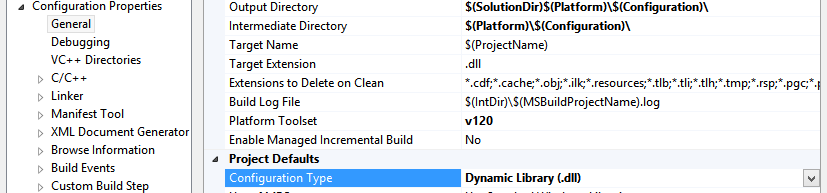
\includegraphics[scale=0.50]{figures/vsdynamiclibrary.png}
  	\caption{Creating a Dynamic Library using Visual Studio}
  	\label{vsdynamiclibrary}
  \end{figure}

 You should then add the \textbf{ws2\_32.lib} and \textbf{q.lib} entries to your Linker inputs in the \verb|Configuration Properties -> Linker -> Input| section.  

	\begin{figure}[H]
		\centering
		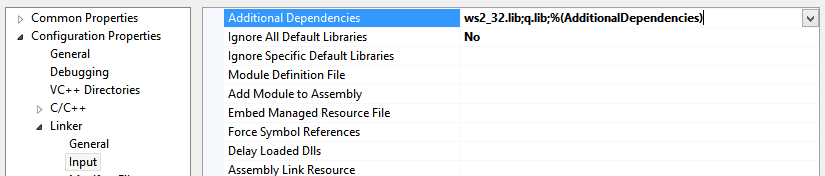
\includegraphics[scale=0.50]{figures/vsdynamiclinker.png}
		\caption{Adding the \textit{ws2\_32.lib} and \textit{q.lib} to the linker inputs using Visual Studio}
		\label{vsdynamiclinker}
	\end{figure}
 
 The \textbf{ws2\_32.lib} is the WinSock2 library and is shipped with Windows, so you don't need to include it in your project. The \textbf{q.lib} file however must be downloaded from the Kx subversion repository and you must ensure that you pick either \textbf{32-bit}\footnote{http://code.kx.com/svn/kx/kdb+/w32/} or \textbf{64-bit}\footnote{http://code.kx.com/svn/kx/kdb+/w64/} depending on which version of kdb+ you are using.
 
 You should now be able to produce a \textbf{.dll} file by adding some basic function definitions and compiling your project. The .dll file will not have any functions in it's symbol table however. This is because Visual Studio, unlike GCC on Linux, will not export any functions into a shared library unless it has been explicitly told to do so. 
 
 You will need to list the functions that are to be made available in your library by creating a \textbf{.def} file or by using the \verb|__declspec|\footnote{https://msdn.microsoft.com/en-us/library/dabb5z75.aspx} attribute syntax. The simplest .def file that will work is just a text file with EXPORTS as the first line followed by the names of any functions that you want to export on following lines. The example below will export the \textit{init} and \textit{halt} functions in the library. This file will also prevent any name mangling that would otherwise occur when compiling these functions (remember that Visual Studio is a C++ compiler!).
 
 \begin{figure}[H]
 \begin{lstlisting}
 EXPORTS
 init
 halt
 \end{lstlisting}
 \caption{A .def file that tells the windows compiler to make the \textit{init} and \textit{halt} functions available in the symbol table}
 \end{figure}
 
 If you are compiling with the \verb|__declspec| declaration on your functions, the names that are exported will be mangled which makes it difficult (if not impossible) to import these functions into kdb+. To solve this, you will also need to prefix your functions with extern "C" to tell the compiler to pass your function names through untouched. It may be helpful to define a macro as below to prefix your functions with to make sure that your API functions are exported correctly.

\begin{figure}[H]
 \begin{lstlisting}
 #define FEEDLIBRARY_API extern "C" __declspec(dllexport)
 
 FEEDLIBRARY_API K init(K x);
 K reload(K x);
 \end{lstlisting}
 \caption{Explicitly making functions visible using the \textit{\_\_declspec} keyword}
 \end{figure}
 
 Examples of using cl.exe to compile code as a dynamically linked library can be found in the
 \textbf{c.a}\footnote{http://code.kx.com/svn/kx/kdb+/c/c/c.a} code sample on the Kx subversion repository.
 
 \subsection{Standalone Executable}
 
 After creating your C++ project in Visual Studio, open the Property Pages and click on \verb|Configuration Properties -> General|. Make sure that the Configuration Type is set to \textbf{Application (.exe)}.
 
 You will need to get the latest \textbf{c.obj} in either the \textbf{w32}\footnote{http://code.kx.com/svn/kx/kdb+/w32} or \textbf{w64}\footnote{http://code.kx.com/svn/kx/kdb+/w64} folders depending on whether you want to create a 32-bit or 64-bit process.
 
The easiest way to make sure that \textbf{c.obj} is added to your project is to navigate to \textit{"Resource Files -> Add... -> Existing Item"} from your solution explorer.
 
 \begin{figure}[H]
 	\centering
 	\fbox{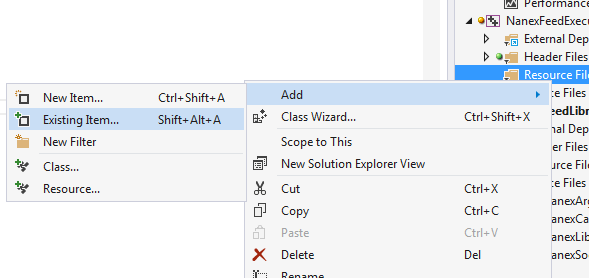
\includegraphics[scale=0.50]{figures/windows_vs2012_static_linking_alt.png}}
 	\caption{Adding an item as a Resource File via the Solution Explorer}
 	\label{addingvsresource}
 \end{figure}
 
 Another way to make sure the objects are included by the linker is to add them to the "Input"
 section of your projects resource page.
 
 \begin{figure}[H]
 	\centering
 	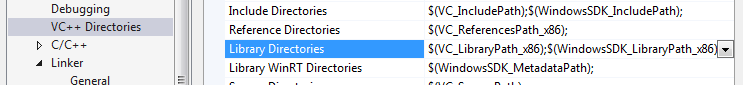
\includegraphics[scale=0.50]{figures/windows_vs2012_static_linking_dirs.png}
 	\caption{Adding an item as a Resource via the Input Resource Page}
 	\label{usingtheinputresourcepage}
 \end{figure}
 
 Note that we add \textbf{ws2\_32.lib} to input section of this page to make sure that the WinSock2 library is included. This file is included on the system path of any recent Windows installation (i.e. Windows XP or greater).
 
 It is also possible to compile the code from the command line on Windows using \textbf{cl.exe}. This can be found by navigating to your Visual Studio installation
 location:
 
 \begin{figure}[H]
 	\begin{lstlisting}
 	C:\Program Files (x86)\Microsoft Visual Studio\12.0\VC\bin.
 	\end{lstlisting}
 	\caption{Location of the cl.exe and msbuild.exe tools}
 \end{figure}
 
 This folder should be added to your system PATH, or you can run \textit{vcvars32.bat} within the same folder in order to make it visible in the current session. The \textbf{c.c}\footnote{http://code.kx.com/svn/kx/kdb+/c/c/c.c} sample hosted in the Kx subversion repository shows how to build an executable using \textbf{cl.exe}.
 
 \section{Loading shared objects into kdb+}
 
 Once you have your shared objects compiled, you should be able to load them into kdb+ using the \textbf{2:}(dynamic load) function\footnote{http://code.kx.com/wiki/Reference/TwoColon}. The example q code below imports three functions: init, find and other from a shared object called example.so. The init and find functions take 0 and 1 arguments respectively. Note that import for the init function declares that it takes 1 argument however! This is because all functions in kdb+ really take at least one argument and that functions with no arguments will be passed a sentinel value instead.
 
 \begin{figure}[H]
 \begin{lstlisting}
 init:`example 2:(`init;1)
 find:`example 2:(`find;1)
 other:`example 2:(`other;3)
 \end{lstlisting}
 \caption{Importing the functions into kdb from a library called example.so using the dynamic load (\textbf{2:}) function.}
 \end{figure}
 
 It is also possible to export these functions from your C code to make it easier to import from kdb+ if you have a large API. You will create a function that returns a dictionary that maps symbols to dynamically loaded functions. An example of such a function is shown below:
 
 \begin{figure}[H]
 \begin{lstlisting}
 K load_funcs(K x)
 {
	 K exportedKeys = ktn(KS, 3);
	 K exportedValues = ktn(0, 3);
 
	 kS(exportedKeys)[0] = ss("init");
	 kS(exportedKeys)[1] = ss("halt");
	 kS(exportedKeys)[2] = ss("get_args");
 
	 kK(exportedValues)[0] = dl(init, 1);
	 kK(exportedValues)[1] = dl(halt, 1);
	 kK(exportedValues)[2] = dl(get_args, 1);
 
	 return xD(exportedKeys, exportedValues);
 }
 \end{lstlisting}
 \caption{A C function that returns a dictionary that maps keys to functions linked using dl}
 \end{figure}
 
 We can then just execute this function from our q script and assign the result to a namespace. \textit{Note that the assignment to the namespace will erase any existing items that were defined in it!}
 
 \begin{figure}[H]
 \begin{lstlisting}
 .fh:(`FeedHandlerLibrary 2:(`load_funcs;1))`
 \end{lstlisting}
 \caption{Loading the function \textit{load\_funcs}, evaluating it, and then assigning the resulting dictionary to a namespace}
 \end{figure}
 
 You should now be able to use the functions from your q script just as you would use any other q function. 
 
 \section{Common Issues}
 
 Some common issues that you may run into when loading shared library functions are:
 
 \begin{description}
 	\item["The symbol is not defined and could not be loaded"] - Either the function has not been exported correctly or there is a typo in the code that loads the function.
 	
 	\item["Incompatible binary format"] - You are trying to load a 32 bit shared library into a 64 bit q process or vice versa.
 \end{description}